\documentclass[preprint]{aastex}
\usepackage{amsmath}
\usepackage{verbatim}
\usepackage{graphicx}
\usepackage{color}
\newcommand{\lnnu}{\ln{\sigma}} 
\usepackage[OT2,T1]{fontenc}
\usepackage{url}

\DeclareSymbolFont{cyrletters}{OT2}{wncyr}{m}{n}
\DeclareMathSymbol{\Sha}{\mathalpha}{cyrletters}{"58}
\begin{document}


\title{Interferometers and Redshift Drift}
This is over an order of magnitude improvement
of the high-precision redshift measurement of  $\sigma_z=6\times 10^{-7}$ obtained
from the radio absorption line in 3C~286 at $z=0.849$
\citep{1978ApJ...219....1D}.

\section{[OII] and [OIII] Emission Line Galaxies as Targets}
Emission line galaxies are excellent candidates for the measurement of precision redshifts.
The unique signature
of doublets amidst  other emission lines allows unambiguous identification of the [OII] $\lambda\lambda$3727--3729\AA\ 
and [OIII]$\lambda\lambda$4959--5007\AA\ doublets.
Their high line fluxes provide strong signals that suppress statistical Poisson uncertainty.
Doublets occupy only a narrow bandwidth that spectrographs must span.
The two lines of a doublet are produced by the same atoms and therefore
share a common line profile: as the wavelength separation of the two lines is proportional to $(1+z)$, their cross-correlation in log-wavelength
provides a measure of redshift that is independent of the specific shape of the line profile.

Potential targets are selected from the Sloan Digital Sky Survey data release SDSS3 DR10.  The  Portsmouth Emission-Line Kinematics table \citep{2013MNRAS.431.1383T}  is used to select
objects 
with $z>0.08$
and sharp and bright [OII] and/or [OIII] emission lines.
The redshifts, velocity dispersions $\Delta v$, line strengths, and host continuum levels for a select set of galaxies are shown in Table~\ref{lines:tab}.
The two-line average $\Delta v$ for [OII] , and the continua flux for bout doublets  are given.
Although we use its velocity dispersions, the Portsmouth table  gives ``rest-frame'' fluxes corrected for dust correction;
the observed fluxes needed to simulate observations are taken from the spZline data model
\citep{2012AJ....144..144B}.  In some cases only one doublet is visible, for example with high-redshift galaxies where [OIII] features are shifted to the near-infrared and are difficult to access from ground-based observations.
A representative 
target, from Plate~\#1268, Fiber~\#318, has its  SDSS spectrum shown in Figure~\ref{shsinput:fig}.

\begin{deluxetable}{cccccccc}
\tablecaption{Target Line Properties.\label{lines:tab}}
\tablehead{
\colhead{} &\colhead{} &\colhead{} &\colhead{}  &\colhead{$\Delta$ v} & \colhead{Flux 1}  & \colhead{Flux 2} & \colhead{Continuum}\\
\colhead{Plate} & \colhead{Fiber} &\colhead{$z$}&\colhead{Doublet} &\colhead{(km\,s$^{-1}$)}& \colhead{(erg\,s$^{-1}$cm$^{-2}$)}& \colhead{(erg\,s$^{-1}$cm$^{-2}$)}& \colhead{(erg\,s$^{-1}$cm$^{-2}$\AA$^{-1}$)}
}
\startdata
1523 & 602 &  0.089 
&[OIII]& $ 5.14$ &$7.04\times 10^{-16}$ &$2.13\times 10^{-15}$ &$1.97\times 10^{-17}$ \\ 
\tableline
1935 & 204 &  0.098 &[OII] & $10.054$ &$1.06\times 10^{-14}$ &$1.28\times 10^{-14}$ &$2.39\times 10^{-16}$\\
&&
&[OIII]& $10.04$ &$1.96\times 10^{-14}$ &$5.93\times 10^{-14}$ &$1.92\times 10^{-16}$ \\ 
\tableline
1036 & 584 &  0.108 
&[OIII]& $ 4.55$ &$3.47\times 10^{-16}$ &$1.05\times 10^{-15}$ &$4.42\times 10^{-17}$ \\ 
\tableline
2959 & 354 &  0.120 
&[OIII]& $ 6.86$ &$1.11\times 10^{-16}$ &$3.36\times 10^{-16}$ &$1.51\times 10^{-18}$ \\ 
\tableline
1268 & 318 &  0.126 &[OII] & $10.044$ &$5.89\times 10^{-15}$ &$6.29\times 10^{-15}$ &$1.77\times 10^{-16}$\\
&&
&[OIII]& $10.04$ &$1.09\times 10^{-14}$ &$3.32\times 10^{-14}$ &$1.46\times 10^{-16}$ \\ 
\tableline
1657 & 483 &  0.221 &[OII] & $10.359$ &$4.69\times 10^{-15}$ &$4.28\times 10^{-15}$ &$1.36\times 10^{-16}$\\
&&
&[OIII]& $10.30$ &$6.07\times 10^{-15}$ &$1.84\times 10^{-14}$ &$1.09\times 10^{-16}$ \\ 
\tableline
1073 & 225 &  0.272 &[OII] & $84.746$ &$8.38\times 10^{-16}$ &$1.05\times 10^{-15}$ &$3.36\times 10^{-17}$\\
&&
&[OIII]& $ 1.43$ &$3.75\times 10^{-16}$ &$1.14\times 10^{-15}$ &$3.89\times 10^{-17}$ \\ 
\tableline
1514 & 137 &  0.318 &[OII] & $10.005$ &$1.20\times 10^{-15}$ &$1.74\times 10^{-15}$ &$6.35\times 10^{-17}$\\
&&
&[OIII]& $10.01$ &$3.85\times 10^{-16}$ &$1.17\times 10^{-15}$ &$1.07\times 10^{-16}$ \\ 
\tableline
4794 & 757 &  0.560 &[OII] & $45.890$ &$2.03\times 10^{-16}$ &$3.18\times 10^{-16}$ &$8.18\times 10^{-18}$\\
&&
&[OIII]& $26.45$ &$8.29\times 10^{-17}$ &$2.51\times 10^{-16}$ &$1.51\times 10^{-17}$ \\ 
\tableline
1059 & 564 &  0.693 &[OII] & $9.580$ &$1.40\times 10^{-17}$ &$1.94\times 10^{-14}$ &$1.47\times 10^{-17}$\\
\tableline

\enddata
\end{deluxetable}


\begin{figure}[t]
   \centering
    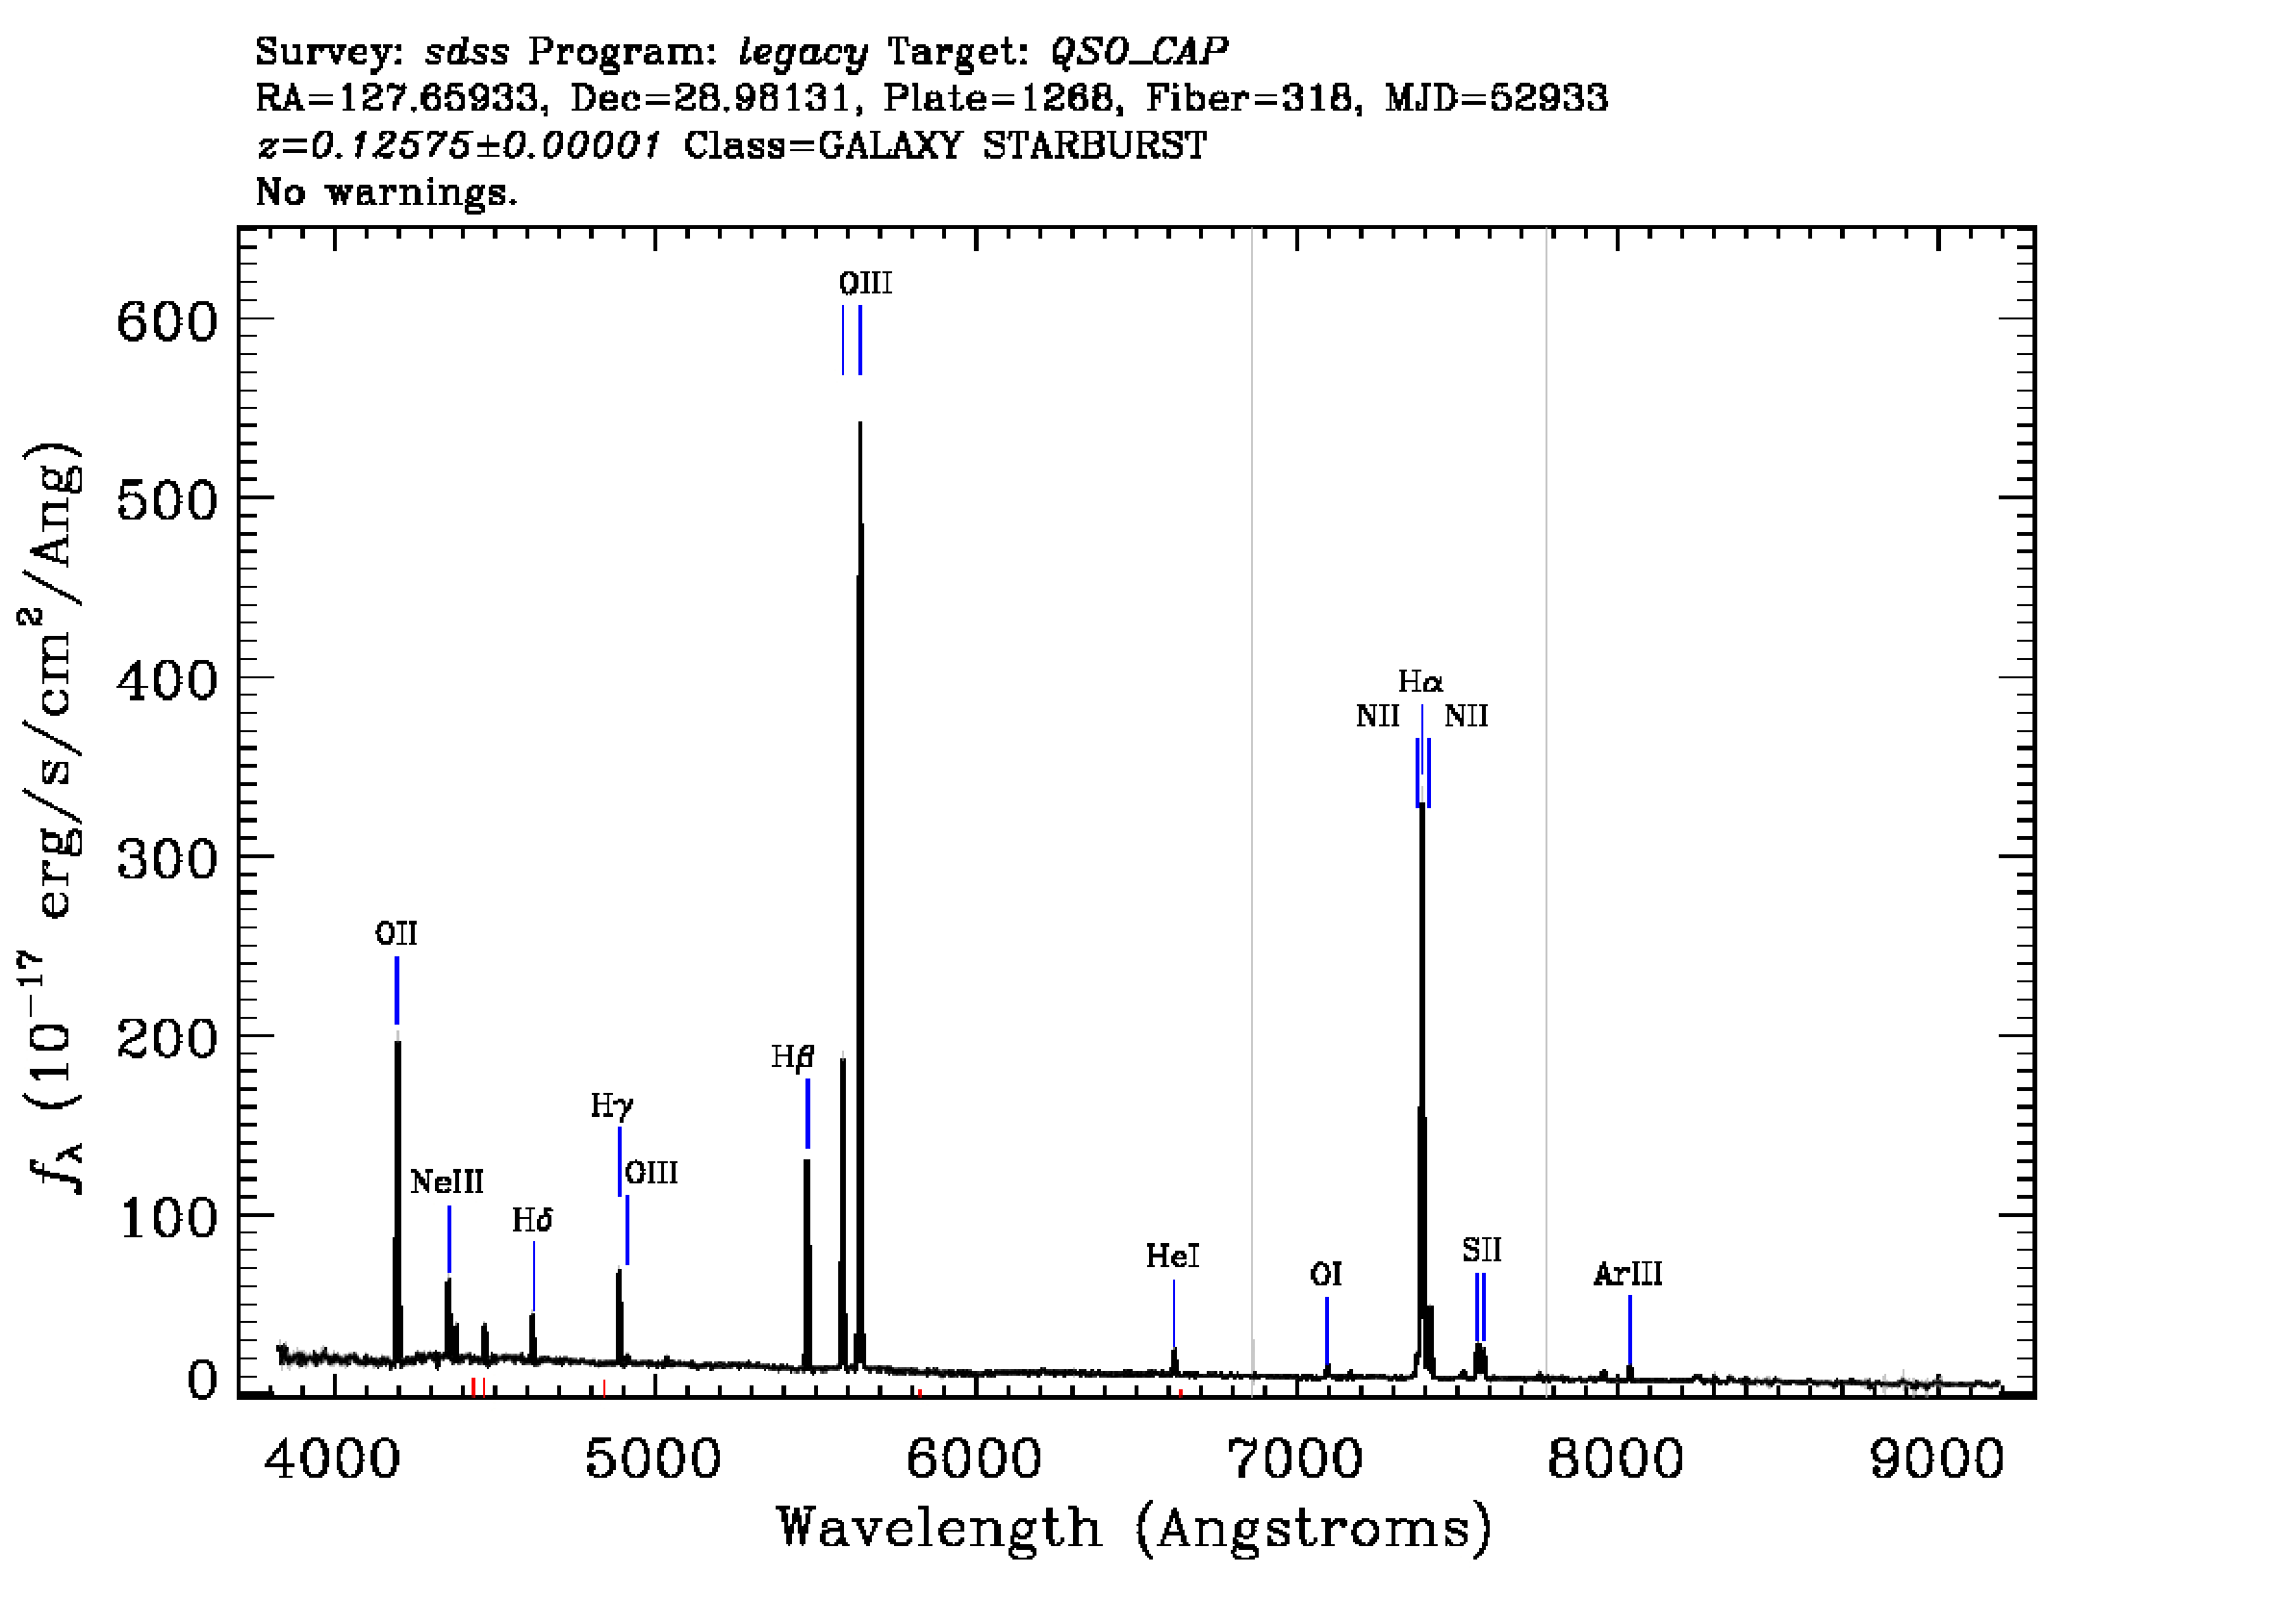
\includegraphics[scale=0.4]{SpecById.pdf} 
  % \plotone{SpecById.eps} 
   \caption{Spectrum of SDSS target specified by Plate~\#1268, Fiber~\#318 from the SDSS3 DR10.  \label{shsinput:fig}}
\end{figure}

The tabulated galaxies are not the product of an exhaustive search and are meant to represent a minimum of what can be available
as good
candidates targets.
Future surveys such as eBOSS, Dark Energy Spectroscopic Instrument, and Euclid will specifically target emission-line
galaxies from which the best targets can be identified.  In the scenarios considered in this article, redshift precision scales
with the inverse of line width and the inverse square of line flux.

The spectral regions of interest
are around each doublet.  In the calculations that follow, these areas are modeled as a function of wavenumber $\sigma$ as
\begin{equation}
B(\sigma)=\frac{a_1}{\sqrt{2\pi s_1^2}}\exp{\left[-\frac{\left(\sigma-\sigma_1\right)^2}{2s_1^2}\right]}+\frac{a_2}{\sqrt{2\pi s_2^2}}\exp{\left[-\frac{\left(\sigma-\sigma_2\right)^2}{2s_2^2}\right]}.
\label{input:eqn}
\end{equation}
The two lines have central wavenumbers $\sigma_1$ and $\sigma_2$, and share a common Gaussian profile with width parameterized by velocity dispersion
such that $s_i=\sigma_i\Delta v/c$. 

\section{Spectrographs Considered For Redshift Measurements}
The precision with which redshift can be determined depends on the instrument used for the measurement.
We consider several spectrometers designs, including a ``Conventional'' high-resolution dispersion spectrograph and the
interferometric instruments ``EDI'',
``SHS'', and ``ED-SHS''.  Interferometers produce a Fourier transform of a signal, converting sharp
spectral features into a wave patterns whose frequency is dependent on the feature wavelength.  Interferometers provide
increased statistical sensitivity to wavelength measurements and potentially have less sensitivity to systematic
uncertainties.

Some common assumptions are made for the spectrometers.
The baseline observation is for an 8-hour exposure on a 10-m telescope.
To allow direct comparison of the 
designs, all systems are assigned the same total throughput of 70\%.
The dispersion spectrometer used for Conventional, EDI, and ED-SHS instruments has $R=20000$ with
point-spread-function dominated by the pixel top-hat function.
For all cases considered photon noise dominates uncertainties, nevertheless
we include a detector read noise of $2e^-$, total integrations split into 2-hour exposures, and a dark current of $2e^-$\,s$^{-1}$. 
Blocking filters remove flux in wavelengths outside the regions
of interest.  The new moon CTIO sky emission is included and
is small compared to the galaxy continuum.
Spatial information is unimportant and the target is considered as point-like: a
circular aperture of $1\arcsec$ diameter is assumed to cover the full line flux.
The effective PSF (including pixels and possible subpixel quantum efficiency variation) 
Nyquist samples the intrinsic line profiles.
When appropriate, the sampling along the spatial axis is not included explicitly in the
signal equations for conciseness.


Projected redshift precisions are calculated with Fisher matrix analysis with the source
redshift $z$ as the only free parameter. 
Precisions scale as the inverse square of exposure time and inverse of telescope aperture. 
For the SHS and when the  $R=20000$ spectrographs resolve the spectral line, the precision scales inversely
with the line dispersion velocity.  
As the measurements
are source-noise dominated, redshift precisions scale as the inverse square of line flux. 

We are interested in uncertainties in redshift drift.  This is in some ways simpler than measuring absolute redshifts
because correlated redshift uncertainties cancel each other when measuring drift.
Instruments contribute sources of measurement uncertainty in redshift drift:  through limitations in the calibration
of wavelength,  uncertainty in the conversion from pixel counts to physical flux, and uncertainty in the point spread function.
Each spectrograph type
has different susceptibilities to  systematic uncertainties.


\subsection{Conventional Dispersion Spectrograph} 
The redshift of a galaxy can be measured from the output of a dispersion spectrograph, such as shown in Figure~\ref{shsinput:fig}.
For an input spectrum $B(\sigma)$ the expected signal is
\begin{equation}
I(\sigma) = \left[B(\sigma)\otimes \mbox{PSF}(\sigma)\right]\Sha\left(\frac{\sigma}{p}\right),
\label{conventional:eqn}
\end{equation}
where $p$ is the spacing of the wavenumber sampling and the Shah function $\Sha$ is the set of delta functions
that specify the discrete sampling,

The wavelengths of the observed lines are compared to the corresponding known restframe to give
the redshift.
\textcolor{red}{Looking into uncertainty of the double wavelengths.
The [OII] double wavelengths are known to $0.0010$\AA\ \citep{1993JPCRD..22.1179M}.}
Projected statistical uncertainties from an $R=20000$ spectrograph for the target galaxies are given under
the ``Conventional'' column of Table~\ref{dz:tab}.  Results from [OII], [OIII], and their combination are listed separately.


\begin{deluxetable}{ccccccc}
\tablecaption{Statistical Uncertainties of Select SDSS Targets With
an 8 Hour Exposure on a 10-m Telescope For Different Spectrographs. \label{dz:tab}}
\tablehead{
\colhead{Plate} &\colhead{Fiber}  &\colhead{Doublet}& \colhead{Conventional} & \colhead{EDI} & \colhead{SHS} &\colhead{ED-SHS}
}
\startdata
1523 & 602 
& OIII  & $1.7\times 10^{-8}$  & $5.8\times 10^{-9}$  & $2.4\times 10^{-8}$  & $5.9\times 10^{-9}$  \\
\tableline
1935 & 204 
& OII & $1.4\times 10^{-8}$  & $4.4\times 10^{-9}$  & $1.7\times 10^{-8}$  & $4.5\times 10^{-9}$  \\
& &OIII  & $6.3\times 10^{-9}$  & $2.1\times 10^{-9}$  & $7.9\times 10^{-9}$  & $2.0\times 10^{-9}$  \\
& &OII\&OIII  & $5.7\times 10^{-9}$  & $1.9\times 10^{-9}$  & $7.2\times 10^{-9}$  & $1.9\times 10^{-9}$  \\
\tableline
1036 & 584 
& OIII  & $2.3\times 10^{-8}$  & $8.8\times 10^{-9}$  & $4.2\times 10^{-8}$  & $7.8\times 10^{-9}$  \\
\tableline
2959 & 354 
& OIII  & $6.0\times 10^{-8}$  & $2.0\times 10^{-8}$  & $9.5\times 10^{-8}$  & $2.1\times 10^{-8}$  \\
\tableline
1268 & 318 
& OII & $1.9\times 10^{-8}$  & $5.7\times 10^{-9}$  & $2.5\times 10^{-8}$  & $6.4\times 10^{-9}$  \\
& &OIII  & $8.6\times 10^{-9}$  & $2.7\times 10^{-9}$  & $1.1\times 10^{-8}$  & $2.8\times 10^{-9}$  \\
& &OII\&OIII  & $7.9\times 10^{-9}$  & $2.4\times 10^{-9}$  & $1.0\times 10^{-8}$  & $2.5\times 10^{-9}$  \\
\tableline
1657 & 483 
& OII & $2.4\times 10^{-8}$  & $7.1\times 10^{-9}$  & $3.1\times 10^{-8}$  & $8.0\times 10^{-9}$  \\
& &OIII  & $1.2\times 10^{-8}$  & $3.9\times 10^{-9}$  & $1.6\times 10^{-8}$  & $4.0\times 10^{-9}$  \\
& &OII\&OIII  & $1.1\times 10^{-8}$  & $3.4\times 10^{-9}$  & $1.4\times 10^{-8}$  & $3.6\times 10^{-9}$  \\
\tableline
1073 & 225 
& OII & $7.2\times 10^{-7}$  & $2.2\times 10^{-7}$  & $8.7\times 10^{-7}$  & $2.3\times 10^{-7}$  \\
& &OIII  & $1.2\times 10^{-8}$  & $6.2\times 10^{-9}$  & $1.3\times 10^{-8}$  & $5.1\times 10^{-9}$  \\
& &OII\&OIII  & $1.2\times 10^{-8}$  & $6.2\times 10^{-9}$  & $1.3\times 10^{-8}$  & $5.1\times 10^{-9}$  \\
\tableline
1514 & 137 
& OII & $4.3\times 10^{-8}$  & $1.4\times 10^{-8}$  & $5.5\times 10^{-8}$  & $1.4\times 10^{-8}$  \\
& &OIII  & $5.6\times 10^{-8}$  & $1.6\times 10^{-8}$  & $1.3\times 10^{-7}$  & $1.8\times 10^{-8}$  \\
& &OII\&OIII  & $3.4\times 10^{-8}$  & $1.0\times 10^{-8}$  & $5.1\times 10^{-8}$  & $1.1\times 10^{-8}$  \\
\tableline
4794 & 757 
& OII & $6.2\times 10^{-7}$  & $1.9\times 10^{-7}$  & $6.6\times 10^{-7}$  & $2.0\times 10^{-7}$  \\
& &OIII  & $4.1\times 10^{-7}$  & $1.3\times 10^{-7}$  & $9.0\times 10^{-7}$  & $1.3\times 10^{-7}$  \\
& &OII\&OIII  & $3.4\times 10^{-7}$  & $1.1\times 10^{-7}$  & $5.3\times 10^{-7}$  & $1.1\times 10^{-7}$  \\
\tableline
1059 & 564 
& OII & $1.7\times 10^{-8}$  & $5.5\times 10^{-9}$  & $1.6\times 10^{-8}$  & $5.6\times 10^{-9}$  \\
\tableline
\enddata
\end{deluxetable}

Not included in Table~\ref{dz:tab} are sources of instrumental systematics.
Wavelength calibration is performed through observations of arc lamps emitting lines at known wavelengths.
The line density is sparse, in that an arc line is not placed on every detector pixel.   If the arc is taken simultaneously
with the science exposure, a minimum wavelength interpolation distance must be maintained so that the arc does
not interfere with the doublet.  Otherwise, the arc must be observed in a different exposure. 
Therefore,  temporal and/or
wavelength interpolation are applied to calibrate wavelengths.

The small number of pixels measuring line flux places stringent requirements on flatfield calibration.  The FWHM of a 10 km\,s$^{-1}$
feature is spanned by 3.15 pixels along the dispersion axis, and (for our calculations) 3 pixels along the spatial axis.
A singe pixel covered by one of the [OIII] lines of the SDSS target specified by Plate~\#1268, Fiber~\#318 has $\sim 10^6$ counts;
in order for photon noise to dominate over pixel flux uncertainty the calibration must be done to significantly better than 0.1\%.

Uncertainty in the often variable and charge-dependent point spread function can
bias the determination of the line centroids.  Just as with the flux calibration requirement, sub-per-mil accuracy in predicted pixel counts
is required.  For redshift drift, these calibration requirements are differential between observations taken
over the duration of the survey: if absolute calibration is not achieved, instrumental stability is essential.


\subsection{Externally Dispersed Interferometer}
The Externally Dispersed Interferometer \citep[EDI;][]{2003PASP..115..255E} is a candidate instrument with which to measure precision redshifts.
An EDI is the sequence of a Fourier transform spectrograph (FTS) and a dispersion spectrograph.  The FTS is an interferometer that shifts
the phase of incoming coherent light
by an amount dependent on wavelength and a  delay between the two arm lengths.
The ensuing dispersion spectrograph takes the phased light and separates it into fine wavelength bins.
For an individual wavelength bin the output signal depends on the phase introduced by the interferometer; multiple
measurements taken after adjusting the delay  make apparent a modulation in the output signals.
Therefore, in an EDI the wavelength can be measured using both the calibration methods of a standard dispersion
spectrograph {\it and} from the modulations of signal apparent when changing the FTS arm-lengths.   As a consequence,
it was shown by
\citet{2003PASP..115..255E} that EDI's provide line-velocity measurements that are more precise than with a dispersion spectrograph.

An EDI produces measurements that can be related
to a conventional spectrum
\begin{equation}
I(\sigma) = B(\sigma) \otimes \mbox{PSF}(\sigma),
\end{equation}
and an independently measurable whirl
\begin{equation}
W(\sigma) = \frac{1}{2}\left[e^{i2\pi\tau_d\sigma}B(\sigma)\right] \otimes \mbox{PSF}(\sigma),
\end{equation}
where $B$ is the input spectrum, $\tau_d$ is the interferometer delay, and $\mbox{PSF}$  is the blurring
response of a pure frequency.

The heterodyning feature of the EDI is seen in the Fourier transforms of the above expressions:
\begin{align}
i(\rho) & =b(\rho) \, \mbox{psf}(\rho)\\
w(\rho -\tau) & =\frac{1}{2} b(\rho) \, \mbox{psf}(\rho-\tau).
\end{align}
The EDI whirl has the instrumental frequency response shifted into a new $\rho$ range to allow
spectral
resolution on scales tuned by the choice of $\tau$.  In the calculations that follow, the delay is chosen to resolve
the FWHM of the line with lower wavenumber, $\tau = (2.36s_1)^{-1}$.

An EDI observation is actually a series of measurements
\begin{equation}
I(\sigma)_{\Delta\tau} = \left[B(\sigma)\left(1+\cos{\left(2\pi\left(\tau+\Delta \tau\right)\sigma+\phi_y \right)} \right)\otimes \mbox{PSF}(\sigma)\right]\Sha\left(\frac{\sigma}{p}\right),
\label{edisig:eqn}
\end{equation}
where $p$ is the spacing of the wavenumber sampling, $\phi_y$ is the initial phase,
and $\Delta \tau$ represents the changes in time delay in the series of exposures; for our calculations we choose  $\Delta \tau = (1+0.25n)\tau $ with $n\in\{0,1,2,3\}$
with the change achieved by adjusting an interferometer arm length.
The first term represents the signal obtained with a conventional spectrograph while the second cosine term
introduces a wavelength-dependent phase that provides additional leverage in measuring redshift.


The expected signal for one of the [OIII] lines of the SDSS target specified by Plate~\#1268, Fiber~\#318 is shown
in Figure~\ref{edicounts:fig}.   In this case the nominal delay is $\tau = 3.57$ mm with measurements
made in steps of 0.892 mm.

\begin{figure}[t]
   \centering
   \plotone{edi.pdf} 
   \caption{The expected EDI signal from the four phase measurements for one of the [OIII] lines of
   the SDSS target specified by Plate~\#1268, Fiber~\#318.
   The four phases parameterized by $n$ is defined in Eqn.~\ref{edisig:eqn}.\label{edicounts:fig}}
\end{figure}


The redshift precisions on the target galaxies are given in Table~\ref{dz:tab}, where each of the four phases receives
a 2-hour exposure.  The EDI performance includes that of the Conventional spectrograph plus
the additional contribution from the whirl; in total the EDI outperforms the Conventional spectrograph
in redshift precision by a factor of $\sim 3$.

Separating the EDI information into Conventional and whirl contributions,
the signal and constraint from the Conventional spectrograph contribution shares those same systematic uncertainties.
The whirl component is best calibrated using arc lamps in the science exposure.  The arc lines determine the configuration
of the EDI itself, $\phi_y$ and the $\Delta \tau$'s, and do not have to be close
to the science lines.  This avoids the temporal and wavelength interpolation needed in conventional spectrographs.
Wavelength uncertainty would then come from mismeasurement of phase and frequency due to pixels local to the
science lines. Absolute flux and PSF uncertainties then become irrelevant.

Flux miscalibration still affect the line profiles, resulting in potential bias in effect wavelength similar to
the Conventional case in scale.  PSF calibration is facilitated with the presence of arc lines from which the
PSF can be directly determined.

\subsection{Spatial Heterodyne Spectroscopy}
\label{SHS:sec}
\subsubsection{Measuring Redshift}
Redshift can also be measured through the sum and the difference of observed wavenumbers of two lines whose restframe wavenumbers are known:
\begin{equation}
(1+z)=\frac{\sigma_{10}+\sigma_{20}}{\sigma_{1}+\sigma_{2}}=\frac{\sigma_{10}-\sigma_{20}}{\sigma_{1}-\sigma_{2}},
\label{redshift:eqn}
\end{equation}
where $\sigma_i$ is the observed and $\sigma_{i0}$ the restframe wavenumber of line $i$.
At face value, the measurement of $\sigma_1\pm\sigma_2$ should be expected to suffer larger uncertainty than that of the wavenumber
of a single line.  To counter this expectation, we consider a scenario where the experimental setup has an output that is naturally sensitive
to $\sigma_1\pm\sigma_2$.  The differential measurement can be immune to certain systematic uncertainties encountered when using dispersion spectrographs.
Redshifts are measured from the relative shift of a single line profile common to two lines of a doublet with no PSF blurring of the
line profiles.



\subsubsection{Signal}
%Specifically,  when using a single feature to measure redshift the shape of the line profile
%contributes uncertainty.
%In contras

We consider Spatial heterodyne spectroscopy (SHS) \citep{1990SPIE.1235..622H}
as a means to get a direct measurement of  $\sigma_1\pm\sigma_2$.
Conceptually, the SHS can be understood as an interferometer with the  mirrors replaced by diffraction gratings.
(Practically we assume an interferometer configuration that  avoids the 50\% light loss inherent to  Michelson interferometers.)
The gratings have line-spacing $d$ and both are tilted
by $\theta$ with respect to the optical axis.  The deflected light from each grating exits the interferometer as a plane wave
propagating with angle $\gamma$ away from the optical axis,  given by the grating equation
\begin{equation}
\sigma\left(\sin{\theta}+\sin{\left(\theta-\gamma\right)}\right)=m/d,
\end{equation}
where $\sigma$ is the wavenumber and $m$ the diffraction order.
The angle of the emergent wave can be re-expressed as
\begin{equation}
\sin{\gamma}=-\cos{\theta} \left(\frac{m}{d\sigma} - \sin{\theta} \right)+ \sin{\theta}\sqrt{1-\left(\frac{m}{d\sigma} -\sin{\theta} \right)^2},
\end{equation}
which is useful in calculations.

The two wavefronts from the two gratings, incident on the detector at angles $-\gamma$ and $\gamma$, interfere to make a fringe
pattern with  frequency
\begin{equation}
f_x=2\sigma\sin{\gamma}.
\end{equation}
For an input spectrum of $B(\sigma)$, the intensity seen at the detector at position $x$ is
\begin{equation}
I(x)=\frac{1}{\Delta x}\left[\int_{0}^{\infty} B(\sigma)\left(1+\cos{\left(2 \pi x (2\sigma \sin{\gamma})\right)}\right)d\sigma \otimes \mbox{PSF}(x)\right]\Sha\left(\frac{x}{p}\right),
\end{equation}
where  $p$ is the spacing of the wavenumber sampling, and for simplicity we assume a square collimated beam that covers
a range  $\Delta x \gg \left(2\sigma \sin{\gamma}\right)^{-1}$.
The Littrow wavenumber $\sigma_0$ is defined such that $2\sigma_0\sin{\theta}=m/d$, $\gamma=0$ and no fringe patterns are produced.

\subsubsection{Toy Example}
\label{toy:sec}
For illustration, consider a toy example where the input signal consists of two $\delta$-functions with the same intensity
\begin{equation}
B(\sigma)=\delta(\sigma_1)+\delta(\sigma_2).
\end{equation}
The output signal density in this case is
\begin{align}
I(x)&=\frac{1}{\Delta x}\left[2+ \cos{\left(2 \pi (2\sigma_1  \sin{\gamma_1}x \right)}+ \cos{\left(2\pi (2  \sigma_2  \sin{\gamma_2})x \right)}\right]\\
&=\frac{2}{\Delta x}\left[1+ \cos{\left(2 \pi  (\sigma_1  \sin{\gamma_1}+ \sigma_2  \sin{\gamma_2})x \right)}\times\cos{\left(2\pi  (\sigma_1  \sin{\gamma_1}- \sigma_2  \sin{\gamma_2})x\right)}\right].
\end{align}
The two mixing of the sinusoidal outputs of the two lines results in two beat frequencies $(\sigma_1  \sin{\gamma_1}\pm\sigma_2  \sin{\gamma_2})$.

When the SHS is configured such that the Littrow wavenumber is
very close to $\sigma_1$ and $\sigma_2$ (and hence $\gamma_1$ and $\gamma_2$
are small),
\begin{equation}
\sigma_{1,2}\sin{\gamma_{1,2}} \approx  2(\sigma_{1,2}-\sigma_0) \tan{\theta}
\end{equation}
and the beat frequencies can be expressed as
$2(\sigma_1+\sigma_2-2\sigma_0)\tan{\theta}$ and $2(\sigma_1-\sigma_2)\tan{\theta}$.
Each beat frequency provides information on either 
$\sigma_1\pm \sigma_2$, the two quantities that directly lead to redshift.

The ratio $n$ between the beat frequencies can be chosen by adjusting the SHS configuration to give
\begin{equation}
\sigma_0=\frac{\sigma_1+\sigma_2}{2}-\frac{\sigma_1-\sigma_2}{2n}.
\label{littrowchoices:eqn}
\end{equation}
For $n=\infty$  the Littrow wavenumber is set to the average of the two lines: $\sigma_0=(\sigma_1+\sigma_2)/2$ and the first beat frequency is zero,
which in practice is difficult to quantify through measurment.  When $n=1$ the Littrow wavenumber is $\sigma_2$, meaning that line produces a flat signal and the other is the source
of the oscillations; the value of the two beat frequencies are equal.


\subsubsection{Performance on Target Galaxies}

We calculate the expected signal using the first order $m=1$ for a SHS with grating line density $1/d=1200$\,mm$^{-1}$
and using the more realistic double line model of Eq.~\ref{input:eqn}
Different configurations of the SHS are achieved by adjusting the grating tilt angle $\theta$, although swapping
gratings can achieve a similar effect.
The SHS configuration can then be expressed in terms of the Littrow wavenumber.

For the [OIII] doublet of the
SDSS target specified by Plate~\#1268, Fiber~\#318 
the condition for having only one beat frequency occurs when $\sigma_0=\sigma_2=17913$\,cm$^{-1}$ and
occurs at $\theta=0.341551$.
Different choices of Littrow wavenumber
produce different output signals:
Figure~\ref{shscounts:fig} shows the expected counts adjusting $\sigma_0$ to produce beat frequency ratios
$n=1/3.5,1/1.05,1,1.05,3.5$ according to Eq.\ \ref{littrowchoices:eqn}.
The maximum $x$ is chosen to be $(12s_1\tan{\theta})^{-1}$ in order to cover the decay caused by the line-width.
The effect on the signal
of the choice of the beat frequency of $2(\sigma_1+\sigma_2-2\sigma_0)\tan{\theta}$ relative to the $2(\sigma_1-\sigma_2)\tan{\theta}$ frequency
is clearly apparent.
The precision is insensitive to the choice of $\sigma_0$, except
for small deviations near $n=1$ and at integer ratios of the beat frequencies; we choose
the case of $n=1.5$ or $\theta = 0.3421194$ (a change in angle of $1.95 \arcmin$ from the $n=1$ case)
as a representative example where the pixels resolve the frequencies of interest.

\begin{figure}[t]
   \centering
   \plotone{shscounts.pdf} 
   \caption{The output signal for positive $x$ of the  SHS configurations that give the four different
   Littrow numbers according to
   $n=1/3.5,1/1.05,1,1.05,3.5$  in Equation~\ref{littrowchoices:eqn}. Only half the signal is shown: it is
   symmetric about $x=0$.\label{shscounts:fig}}
\end{figure}

The redshift precisions on the target galaxies are given in Table~\ref{dz:tab}.  The statistical uncertainties are slightly worse than for
the Conventional spectrograph and well below EDI.  However, the results have reduced sensitivity to PSF uncertainties.

Wavelength calibration is tied to the determination of the EDI system parameters, the grating density $1/d$ and angle $\theta$.
Both can be calibrated externally through direct measurements, or arc lamp exposures; including lamp light
in science exposures is not preferred as all sources of light contribute the noise background.
Alternatively
the long exposures can be divided into sub-exposures each with a different SHS configuration, either by changing the
gratings or by rotating the grating angles by a series of $\delta \theta$.  The data themselves can be then used to fit for
the hardware parameters.

The line signal is distributed over thousands of pixels reducing the pixel flux requirement to better than 1\%, much less stringent
than for the the Conventional and EDI spectrographs.

Converting the spectrum to Fourier space transforms the sharp imperfectly-known line profiles into the low-frequency envelope,
distinct from the high-frequency wiggles characteristic to each configuration that inform the redshift measurement.
The PSF blurring applies not in wavenumber space where it affects
line shapes but rather in physical space after the conversion of the lines into cosine functions; the PSF does not directly bias the effective
wavelength of lines.

\subsection{ED-SHS}
The two doublet lines combine to produce a mixed signal in an SHS.  Sending SHS light, such as those signals shown
in  Figure~\ref{shscounts:fig}, into an ensuing dispersion grating
allows the disentangling of the two signals for an unambiguous measure of the frequency of each.  In this article,
this scheme is 
referred to as an External Dispersion SHS (ED-SHS).
The observed signal is described by
\begin{equation}
I(\sigma,x) = \frac{1}{\Delta x}\left[\int^{\sigma \exp{\left(1/2R\right)}}_{\sigma} B(\sigma')\left(1+\cos{\left(2 \pi x (2\sigma' \sin{\gamma})\right)}\right)d\sigma' \otimes \mbox{PSF}(\sigma,x)\right]\Sha\left(\frac{\sigma}{p_\sigma}\right) \Sha\left(\frac{x}{p_x}\right).
\label{edishssig:eqn}
\end{equation}
The similarities between ED-SHS and EDI can be seen in Fig,\ 2 of \citet{2003PASP..115..255E}; both use
interferometry to create wavelength-dependent modulations in the signal, the distinction between the two coming
from the functional form of
the modulation frequency.


The signal from two columns of pixels corresponding to the two wavelengths of
the [OIII] doublet of the
SDSS target specified by Plate~\#1268, Fiber~\#318 is shown in Figure~\ref{edshs:fig}.
The Littrow wavelength is set to the average of the two lines  $\sigma_0=(\sigma_1+\sigma_2)/2$.
In an SHS the output signal would be the sum of these and all other columns in the bandpass.

\begin{figure}[t]
   \centering
   \plotone{edshs} 
   \caption{The output signal for positive $x$ of the  SHS configuration
    $\sigma_0=(\sigma_1+\sigma_2)/2$. \label{edshs:fig}}
\end{figure}

The redshift precisions on the target galaxies are given in Table~\ref{dz:tab}.  The statistical uncertainties are improved compared to those of the
SHS, and are comparable to the performance of the EDI.

Now that the signals from different wavelengths are no longer mixed, calibration arcs can be observed with the science image without increasing
the photon noise of the doublet lines.  Both wavelength and PSF calibration are simplified as with the EDI.
In addition, the flux signals are further reduced relative to the SHS relaxing flux calibration requiirements.

\subsection{Misc}
Maybe these instruments are good for atomic line catalogs.

\bibliographystyle{apj}
\bibliography{/Users/akim/Documents/alex.bib}

\end{document}
